\subsection{Bediensoftware}%Elias 1 Seite
%Topdown beschreibung
Als Bediensoftware wurde ein Java-Applikation geschrieben. Diese soll den Benutzern die Möglichkeit bieten, die gemessenen Daten auszulesen und in ein gebräuchliches Format zu exportieren. Das eine einfache Weiterverarbeitung der Daten ermöglicht beispielsweise in Excel oder Matlab.

Das Programm bietet drei Hauptfunktionen um mit dem P3T7 zu kommunizieren. Diese sind im Bereich 'Steuerung' zu finden. Daneben bietet das Tool die Funktion sich mit dem P3T7 zu verbinden. Die im Bereich 'Bluetooth' zu finden ist. Die restlichen Elemente dienen alle der Ausgabe. Der 'Status' visualisiert den Fortschritt des Downloads. Im Bereich 'Echtzeit' werden die aktuellen Messwerte des P3T7 angezeigt. Im dominierenden Bereich 'Plot' werden die Daten aus dem Speicher visualisiert, um dem Benutzer eine schnelle Validierung der Daten zu ermöglichen.

\begin{figure}[H]
\begin{center}
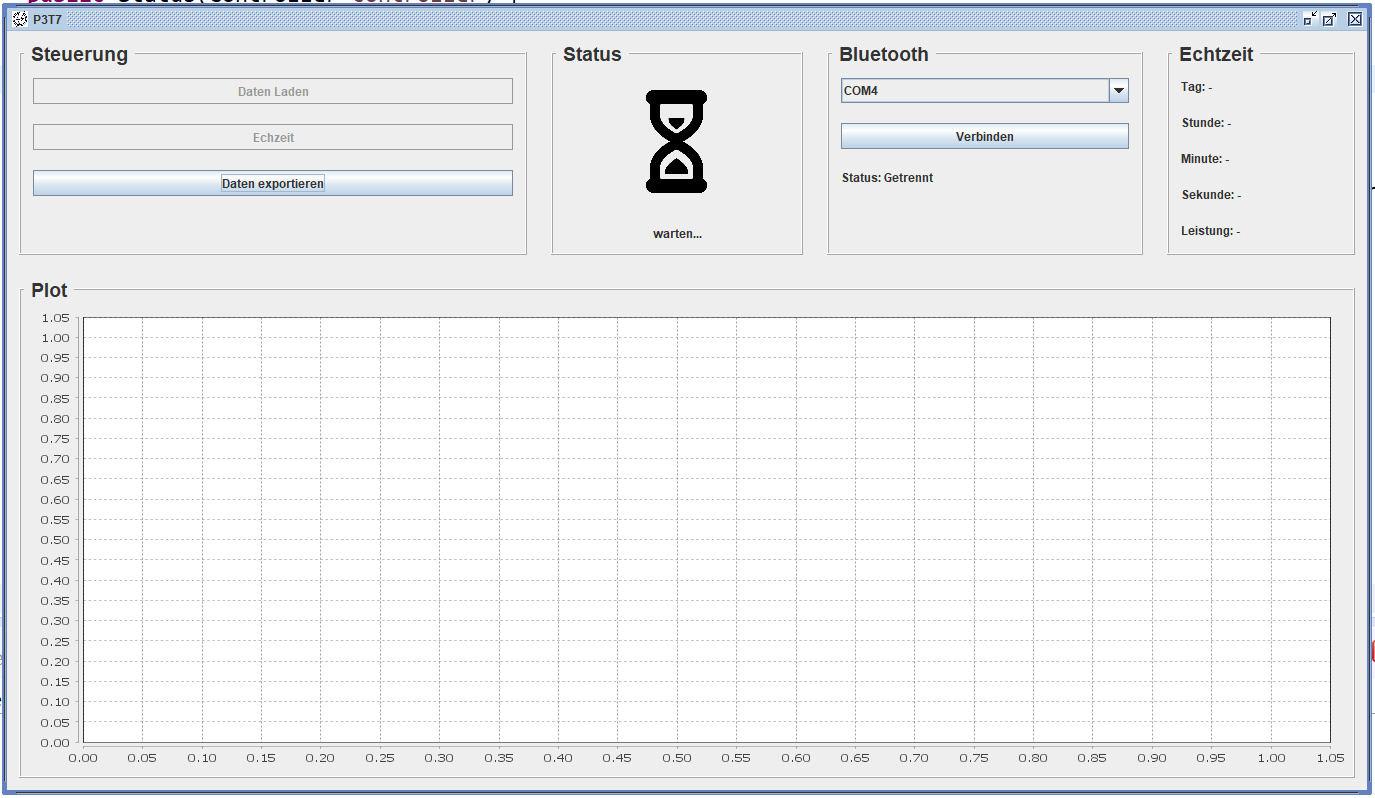
\includegraphics[width=0.9\textwidth]{images/Software_GUI.png}
\caption{GUI der Bediensoftware}
\end{center}
\end{figure}

\subsubsection*{Steuerung}

Mit den drei Hauptfunktionen können die Daten aus dem P3T7 extrahiert werden. Wenn ein Download gestartet wird, kann auf dem Status-Panel der Fortschritt beobachtet werden. Falls der Download abgeschlossen ist werden die Daten im Plot dargestellt. Dieser soll dem Nutzer die Sicherheit geben, dass keine falschen Daten heruntergeladen wurden. Anschliessend kann mit dem Button 'Daten exportiern' ein CSV-File generiert werden. Dieses ist mit dem Namen 'ausgabe.txt' neben der Programmdatei zu finden. Mit dem Button 'Echtzeit' kann die Echtzeitübertragung gestartet werden. Während der Echtzeitübertragung wird jede Sekunde die aktuellen Messwerte an das Tool weitergeleitet. Diese werden anschliessend direkt im Echtzeit-Panel angezeigt.

\subsubsection*{Bluetooth}

Das Bluetoot-Modul emuliert über Bluetooth eine seriell Verbindung. Um das Tool mit dem P3T7 zu verbinden muss zuerst im Betriebssystem das P3T7 gekoppelt werden.  Ist dies erfolgt kann im Tool im Bluetooth-Panel aus dem Dropdown-Menu der entsprechende ComPort ausgewählt werden. Dieser kann im Gerätemanager nachgeschaut werden. Falls ein falscher Port ausgewählt wird vergeht eine Zeit(ca. 30s) bis das Programm den Fehler bemerkt, welche abgewartet wird.


\subsubsection*{Programmstruktur}

Das Programm wurde nach dem MVC Pattern realisiert. Somit hat es praktisch keine nennenswerten strukturellen Eigenheiten bis auf das Interface für die serielle Verbindung. 

\begin{figure}[H]
\begin{center}
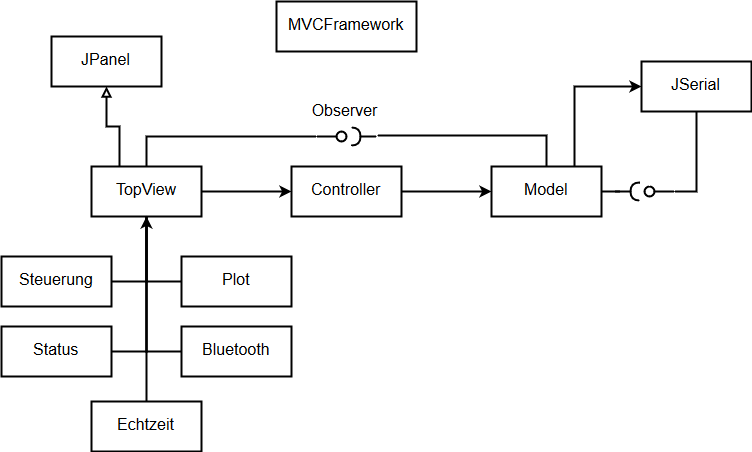
\includegraphics[width=0.9\textwidth]{images/Software_UML.png}
\caption{UML Diagramm der Bediensoftware}
\end{center}
\end{figure}

